\section{DẤU TAM THỨC BẬC HAI}
\subsection{TÓM TẮT LÝ THUYẾT}
\subsubsection{Dấu của tam thức bậc hai}
\begin{itemize}
	\item [\iconMT] \indam{Định nghĩa:}  Tam thức bậc hai (đối với $x$ ) là biểu thức có dạng $f(x)=ax^2+bx+c$. Trong đó $a, b, c$ là những số cho trước với $a\ne 0$.
	
	\begin{boxkn}
		\begin{itemize}
			\item Nghiệm của phương trình $ax^2+bx+c=0$ được gọi là nghiệm của tam thức bậc hai.
			\item $ \Delta =b^2-4ac$ và $ \Delta '=b'^2-ac$ theo thứ tự được gọi là biệt thức và biệt thức thu gọn của tam thức bậc hai.
		\end{itemize}
	\end{boxkn}
	\item [\iconMT] \indam{Định lý về dấu của tam thức bậc hai: } Ta đã biết hàm số $y=ax^2+bx+c$ với $a \ne 0$ có đồ thị là một parabol.
	\begin{itemize}
		\item [\iconCH] Nếu $a>0$, ta có các trường hợp sau:\\
		\begin{tcolorbox}[colframe=orange,colback=orange!4,boxrule=0.2mm]
				\begin{minipage}{4cm}
				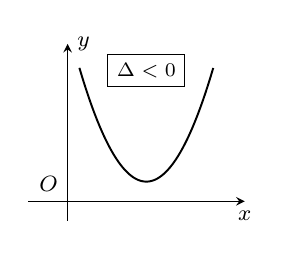
\begin{tikzpicture}[smooth,samples=300,scale=0.5,>=stealth,font=\footnotesize]
					\draw[->] (-1,0)--(4.5,0) node[below]{$x$};
					\draw[->] (0,-0.5)--(0,4) node[right]{$y$};
					\draw (0,0) node[above left]{$O$};
					\draw[line width=0.7pt,domain=0.3:3.7] plot(\x,{(\x)^2-4*(\x)+4.5});
					\node[below] at (2,4) {\fbox{\scriptsize$\Delta <0$}};
				\end{tikzpicture}\\
				\indamm{Đồ thị luôn nằm trên $Ox$.}
			\end{minipage}\hspace{1cm}
			\begin{minipage}{4cm}
				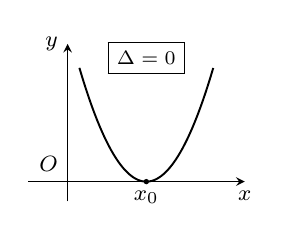
\begin{tikzpicture}[smooth,samples=300,scale=0.5,>=stealth,font=\footnotesize]
					\draw[->] (-1,0)--(4.5,0) node[below]{$x$};
					\draw[->] (0,-0.5)--(0,3.5) node[left]{$y$};
					\draw (0,0) node[above left]{$O$};
					\draw[line width=0.7pt,domain=0.3:3.7] plot(\x,{(\x)^2-4*(\x)+4});
					\draw[fill=black] (2,0) circle(1.5pt);
					\node[below] at (2,0) {$x_0$};
					\node[below] at (2,3.8) {\fbox{\scriptsize$\Delta =0$}};
				\end{tikzpicture}\\
				\indamm{Đồ thị nằm trên $Ox$ khi $x \ne x_0=-\frac{b}{2a}$.}
			\end{minipage}\hspace{1cm}
			\begin{minipage}{4cm}
				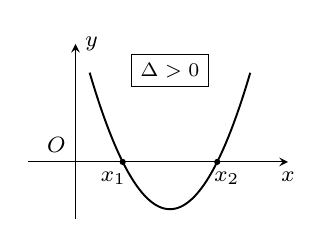
\begin{tikzpicture}[smooth,samples=300,scale=0.6,>=stealth,font=\footnotesize]
					\draw[->] (-1,0)--(4.5,0) node[below]{$x$};
					\draw[->] (0,-1.2)--(0,2.5) node[right]{$y$};
					\draw (0,0) node[above left]{$O$};
					\draw[line width=0.7pt,domain=0.3:3.7] plot(\x,{(\x)^2-4*(\x)+3});
					\draw[fill=black] (1,0) circle(1.5pt) (3,0) circle(1.5pt);
					\node[below] at (0.8,0) {$x_1$};
					\node[below] at (3.2,0) {$x_2$};
					\node[below] at (2,2.5) {\fbox{\scriptsize$\Delta >0$}};
				\end{tikzpicture}\\
				\indamm{Đồ thị nằm trên $Ox$ khi $x<x_1$ hoặc $x>x_2$; nằm dưới $Ox$ khi $x_1<x<x_2$.}
			\end{minipage}
		\end{tcolorbox}
		
		\item [\iconCH] Nếu $a<0$:, ta có các trường hợp sau:\\
		\begin{tcolorbox}[colframe=orange,colback=orange!4,boxrule=0.2mm]
		\begin{minipage}{4cm}
			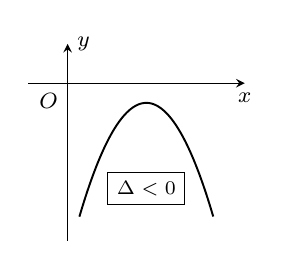
\begin{tikzpicture}[smooth,samples=300,scale=0.5,>=stealth,font=\footnotesize]
				\draw[->] (-1,0)--(4.5,0) node[below]{$x$};
				\draw[->] (0,-4)--(0,1) node[right]{$y$};
				\draw (0,0) node[below left]{$O$};
				\draw[line width=0.7pt,domain=0.3:3.7] plot(\x,{-(\x)^2+4*(\x)-4.5});
				\node[below] at (2,-2) {\fbox{\scriptsize$\Delta <0$}};
			\end{tikzpicture}\\
		\indamm{Đồ thị luôn nằm dưới $Ox$.}
		\end{minipage}\hspace{1cm}
		\begin{minipage}{4cm}
			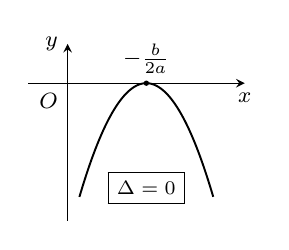
\begin{tikzpicture}[smooth,samples=300,scale=0.5,>=stealth,font=\footnotesize]
				\draw[->] (-1,0)--(4.5,0) node[below]{$x$};
				\draw[->] (0,-3.5)--(0,1) node[left]{$y$};
				\draw (0,0) node[below left]{$O$};
				\draw[line width=0.7pt,domain=0.3:3.7] plot(\x,{-(\x)^2+4*(\x)-4});
				\draw[fill=black] (2,0) circle(1.5pt);
				\node[above] at (2,0) {$-\frac{b}{2a}$};
				\node[below] at (2,-2) {\fbox{\scriptsize$\Delta =0$}};
			\end{tikzpicture}\\
		\indamm{Đồ thị nằm dưới $Ox$ khi $x \ne x_0=-\frac{b}{2a}$.}
		\end{minipage}\hspace{1cm}
		\begin{minipage}{4cm}
			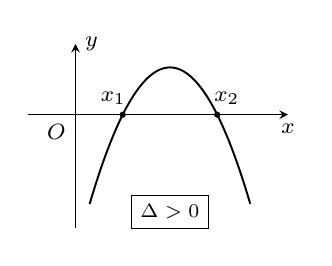
\begin{tikzpicture}[smooth,samples=300,scale=0.6,>=stealth,font=\footnotesize]
				\draw[->] (-1,0)--(4.5,0) node[below]{$x$};
				\draw[->] (0,-2.4)--(0,1.5) node[right]{$y$};
				\draw (0,0) node[below left]{$O$};
				\draw[line width=0.7pt,domain=0.3:3.7] plot(\x,{-(\x)^2+4*(\x)-3});
				\draw[fill=black] (1,0) circle(1.5pt) (3,0) circle(1.5pt);
				\node[above] at (0.8,0) {$x_1$};
				\node[above] at (3.2,0) {$x_2$};
				\node[below] at (2,-1.5) {\fbox{\scriptsize$\Delta >0$}};
			\end{tikzpicture}\\
		\indamm{Đồ thị nằm dưới $Ox$ khi $x<x_1$ hoặc $x>x_2$; nằm trên $Ox$ khi $x_1<x<x_2$.}
		\end{minipage}
		\end{tcolorbox}
	\end{itemize}
\end{itemize}
Tương ứng hình ảnh đồ thị ở trên, ta có bảng tổng kết dấu của tam thức bậc hai như sau:
\begin{itemize}
	\item [\iconCH] Nếu $a>0$:
	\begin{listEX}[3]
		\item [] 
\begin{tikzpicture}[scale=0.8,font=\footnotesize]
			\tkzTabInit[nocadre=false,lgt=1,espcl=2.5]
			{$x$ /0.6,$f(x)$ /0.6}
			{$-\infty$,$+\infty$}
			\tkzTabLine{,+,}
		\end{tikzpicture}
		\item [] 
\begin{tikzpicture}[scale=0.8,font=\footnotesize]
			\tkzTabInit[nocadre=false,lgt=1,espcl=1.4]
			{$x$ /0.6,$f(x)$ /0.6}
			{$-\infty$,$x_0$,$+\infty$}
			\tkzTabLine{,+,$0$,+,}
		\end{tikzpicture}
		\item [] 
\begin{tikzpicture}[scale=0.8,font=\footnotesize]
			\tkzTabInit[nocadre=false,lgt=1,espcl=1.2]
			{$x$ /0.6,$f(x)$ /0.6}
			{$-\infty$,$x_1$,$x_2$,$+\infty$}
			\tkzTabLine{,+,$0$,-,$0$,+,}
		\end{tikzpicture}
	\end{listEX}
	\item [\iconCH] Nếu $a<0$:
	\begin{listEX}[3]
		\item [] 
\begin{tikzpicture}[scale=0.8,font=\footnotesize]
			\tkzTabInit[nocadre=false,lgt=1,espcl=2.5]
			{$x$ /0.6,$f(x)$ /0.6}
			{$-\infty$,$+\infty$}
			\tkzTabLine{,-,}
		\end{tikzpicture}
		\item [] 
\begin{tikzpicture}[scale=0.8,font=\footnotesize]
			\tkzTabInit[nocadre=false,lgt=1,espcl=1.4]
			{$x$ /0.6,$f(x)$ /0.6}
			{$-\infty$,$x_0$,$+\infty$}
			\tkzTabLine{,-,$0$,-,}
		\end{tikzpicture}
		\item [] 
\begin{tikzpicture}[scale=0.8,font=\footnotesize]
			\tkzTabInit[nocadre=false,lgt=1,espcl=1.2]
			{$x$ /0.6,$f(x)$ /0.6}
			{$-\infty$,$x_1$,$x_2$,$+\infty$}
			\tkzTabLine{,-,$0$,+,$0$,-,}
		\end{tikzpicture}
	\end{listEX}
\end{itemize}
\newpage
\begin{minipage}{8cm}
	\begin{tcolorbox}[colframe=cyan,colback=cyan!3,boxrule=0.2mm]
		\indamm{Định lý về dấu tam thức bậc hai:} Cho tam thức bậc hai $f(x)=ax^2+b x+c\,(a \neq 0)$.
		\begin{itemize}
			\item [\iconCH] Nếu $\Delta<0$ thì $f(x)$ cùng dấu với hệ số $a$ với mọi $x \in \mathbb{R}$.
			\item [\iconCH] Nếu $\Delta=0$ thì $f(x)$ cùng dấu với hệ số $a$ với mọi $x \neq-\frac{b}{2 a}$.
			\item [\iconCH] Nếu $\Delta>0$ thì tam thức $f(x)$ có hai nghiệm phân biệt $x_1$ và $x_2$ $\left(x_{1}<x_{2}\right)$. Khi đó, $f(x)$ cùng dấu với hệ số $a$ với mọi $x \in\left(-\infty ; x_{1}\right) \cup\left(x_{2} ;+\infty\right) ; f(x)$ trái dấu với hệ số $a$ với mọi $x \in\left(x_{1} ; x_{2}\right)$
		\end{itemize}
	\end{tcolorbox}
\end{minipage}\hspace{0.5cm}
\begin{minipage}{9cm}
\begin{khung4}{Ghi nhớ dấu của $f(x)$ và $a$}
\begin{itemize}
	\item[\iconCH] Nếu $\Delta < 0$ thì\\
		\begin{tikzpicture}
			\tkzTabInit[nocadre=false,lgt=1.2,espcl=4.2]
			{$x$ /0.7,$f(x)$ /0.8}
			{$-\infty$,$+\infty$}
			\tkzTabLine{,\text{cùng dấu },}
		\end{tikzpicture}
	\item[\iconCH] Nếu $\Delta = 0$ thì\\
		\begin{tikzpicture}
			\tkzTabInit[nocadre=false,lgt=1.2,espcl=2.5]
			{$x$ /0.7,$f(x)$ /0.8}
			{$-\infty$,$-\frac{b}{2a}$,$+\infty$}
			\tkzTabLine{,\text{cùng dấu },$0$,\text{ cùng dấu },}
		\end{tikzpicture}
	\item[\iconCH] Nếu $\Delta > 0$ thì\\
		\begin{tikzpicture}
		\tkzTabInit[nocadre=false,lgt=1.2,espcl=1.7]
		{$x$ /0.7,$f(x)$ /1}
		{$-\infty$,$x_1$,$x_2$,$+\infty$}
		\tkzTabLine{,\text{cùng dấu },$0$,\text{ trái dấu },$0$,\text{ cùng dấu },}
	\end{tikzpicture}
\end{itemize}
\end{khung4}
\end{minipage}

\subsubsection{Bất phương trình bậc hai}
\begin{itemize}
	\item [\iconMT] \indam{Định nghĩa:} Bất phương trình bậc hai ẩn $x$ là bất phương trình có dạng $a x^{2}+b x+c>0$ (hoặc $\left.a x^{2}+b x+c \geq 0, a x^{2}+b x+c<0, a x^{2}+b x+c \leq 0\right)$, trong đó $a, b, c$ là những số thực đã cho và $a \neq 0$.
	\begin{boxkn}
	\begin{itemize}
		\item Số thực $x_{0}$ gọi là một nghiệm của bất phương trình bậc hai $a x^{2}+b x+c>0$, nếu $a x_{0}^{2}+b x_{0}+c>0$. Tập hợp gồm tất cả các nghiệm của bất phương trình bậc hai $a x^{2}+b x+c>0$ gọi là tập nghiệm của bất phương trình này.
		\item Giải một bất phương trình bậc hai là tìm tập nghiệm của nó.
	\end{itemize}
\end{boxkn}
	\item [\iconMT] \indam{Một số kết quả cần nhớ:} Cho tam thức bậc hai $ax^2+bx+c$, với $a \ne 0$.
	\begin{listEX}[2]
		\item [\ding{172}]$ax^2+bx+c>0, \forall x\in \mathbb{R} \Leftrightarrow \left\{\begin{aligned}
			&a>0\\
			& \Delta <0.
		\end{aligned}\right.$
		\item [\ding{173}] $ax^2+bx+c<0, \forall x\in \mathbb{R} \Leftrightarrow \left\{\begin{aligned}
			&a<0\\
			& \Delta <0.
		\end{aligned}\right. $
		\item [\ding{174}] $ax^2+bx+c\geqslant 0, \forall x\in \mathbb{R} \Leftrightarrow \left\{\begin{aligned}
			&a>0\\
			& \Delta \leqslant 0.
		\end{aligned}\right. $
		\item [\ding{175}] $ax^2+bx+c\leqslant 0, \forall x\in \mathbb{R} \Leftrightarrow \left\{\begin{aligned}
			&a<0\\
			& \Delta \leqslant 0.
		\end{aligned}\right. $
	\end{listEX}
\end{itemize}

\subsection{RÈN LUYỆN KĨ NĂNG GIẢI TOÁN}
\begin{dang}{Xét dấu tam thức bậc hai $f(x)=ax^2+bx+c$, với $a \ne 0$}
	\begin{itemize}
		\item [$\bullet$] Tìm nghiệm $ax^2+bx+c=0 \quad (1)$.
		\item [$\bullet$] Tùy thuộc vào số nghiệm của (1), ta lựa chọn bảng xét dấu phù hợp.
	\end{itemize}
\begin{note}
	Ghi nhớ ngắn gọn: Nếu $\Delta \le 0$ thì cùng dấu $a$; Nếu $\Delta >0 $ thì  "trong trái, ngoài cùng".
\end{note}
\end{dang}

\begin{vd}%[0D4Y5-1]
	Xét dấu của các tam thức sau
	\begin{listEX}[3]
		\item $3x^2-2x+1$.
		\item $-x^2+4x+5$.
		\item $4x^2+4x+1$.
		\item $2x^2 - 6x + \dfrac{9}{2}$.
		\item $3x^2 - 2x - 8$ .
		\item $- x^2 + 2x - 1$.
	\end{listEX}
	\loigiai{
		\begin{listEX}
			\item Ta có $ \Delta '=-2<0$ và $a=3>0$. Suy ra $3x^2-2x+1>0,\forall x\in \mathbb{R}$.
			\item Ta có $-x^2+4x+5=0 \Leftrightarrow \left[\begin{aligned}& x=-1 \\ & x=5.\end{aligned}\right. $\\
			Bảng xét dấu
			\begin{center}
				\begin{tikzpicture}
					\tkzTabInit[lgt=3,espcl=2]
					{$x$ /0.8, $-x^2+4x+5$ /0.8}
					{$-\infty$,$-1$,$5$,$+\infty$}
					\tkzTabLine{ ,-,$0$,+,$0$,-,}
				\end{tikzpicture}
			\end{center}
			Suy ra $-x^2+4x+5>0 \Leftrightarrow x\in (-1;5)$ và $-x^2+4x+5<0 \Leftrightarrow x\in (-\infty;-1)\cup (5;+\infty)$.
			\item Tam thức bậc hai $f(x)=4x^2+4x+1$ có $\Delta=0$, nghiệm kép $x_0=-\dfrac{1}{2}$ và hệ số $a=4>0$ nên $f(x)>0$ với mọi $x\in\mathbb{R}\setminus\left\{-\dfrac{1}{2}\right\}$.
			\item Ta có $f(x)=0\Leftrightarrow 2x^2-6x+\dfrac{9}{2}=0\Leftrightarrow x=\dfrac{3}{2}$.\\ Bảng xét dấu
			\begin{center}
				
\begin{tikzpicture}
					\tkzTabInit[nocadre=false,lgt=1.2,espcl=4,deltacl=0.6] %phần bắt buộc
					{$x$ /1,$f(x)$ /0.6}
					{$-\infty$,$\dfrac{3}{2}$,$+\infty$}
					\tkzTabLine{,+,$0$,+,}
				\end{tikzpicture}
			\end{center}
			\item Ta có $f(x)=0\Leftrightarrow 3x^2-2x-8=0\Leftrightarrow \hoac{& x=-\dfrac{4}{3} \\ & x=2}$.\\ Bảng xét dấu
			\begin{center}
				
\begin{tikzpicture}
					\tkzTabInit[nocadre=false,lgt=1.2,espcl=2.5,deltacl=0.6] %phần bắt buộc
					{$x$ /1,$f(x)$ /0.6}
					{$-\infty$,$-\dfrac{4}{3}$,$2$,$+\infty$}
					\tkzTabLine{,+,$0$,-,$0$,+,}
				\end{tikzpicture}
			\end{center}
			\item Ta có $f(x)=0\Leftrightarrow -x^2+2x-1=0\Leftrightarrow x=1$.\\ Bảng xét dấu
			\begin{center}
				
\begin{tikzpicture}
					\tkzTabInit[nocadre=false,lgt=1.2,espcl=4,deltacl=0.6] %phần bắt buộc
					{$x$ /1,$f(x)$ /0.6}
					{$-\infty$,$1$,$+\infty$}
					\tkzTabLine{,-,$0$,-,}
				\end{tikzpicture}
			\end{center}
		\end{listEX}
	}
\end{vd}
\begin{vd}%[0D4B5-1]
	Tìm nghiệm và lập bảng xét dấu của tam thức bậc hai $f(x)$ với đồ thị được cho ở mỗi hình\\
	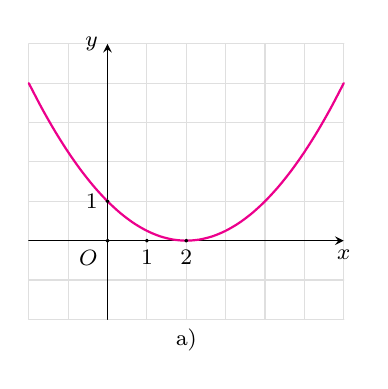
\begin{tikzpicture}[scale=.5, font=\footnotesize, line join=round, line cap=round, >=stealth]
		\draw[gray!50,opacity=.5](-2,-2)grid(6,5);
		\draw[->](-2,0)--(0,0)node[below left]{$O$}--(6,0)node[below]{$x$};
		\draw[->](0,-2)--(0,5)node[left]{$y$};
		\draw[smooth,domain=-2:6,thick,magenta]plot(\x,{1/4*(\x)^2-(\x)+1});
		\draw (2,-2)node[below]{a)};
		\draw(1,0)node[below]{$1$};
		\draw(2,0)node[below]{$2$};
		\draw(0,1)node[left]{$1$};
		\foreach \x in{0,1,2}\draw[fill](\x,0)circle(1pt);
		\draw[fill](0,1)circle(1pt);
		
	\end{tikzpicture}\hspace*{1cm}
	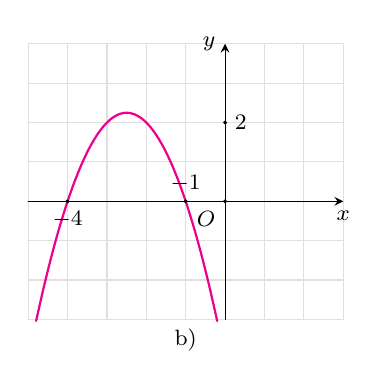
\begin{tikzpicture}[scale=.5, font=\footnotesize, line join=round, line cap=round, >=stealth]
		\draw[gray!50,opacity=.5](-5,-3)grid(3,4);
		\draw[->](-5,0)--(0,0)node[below left]{$O$}--(3,0)node[below]{$x$};
		\draw[->](0,-3)--(0,4)node[left]{$y$};
		\draw[smooth,domain=-4.8:-0.2,thick,magenta]plot(\x,{-(\x)^2-5*(\x)-4});
		\draw (-1,-3)node[below]{b)};
		\draw(-4,0)node[below]{$-4$};
		\draw(0,2)node[right]{$2$};
		\draw(-1,0)node[above]{$-1$};
		\foreach \x in{-4,-1,0}\draw[fill](\x,0)circle(1pt);
		\draw[fill](0,2)circle(1pt);
		
	\end{tikzpicture}\hspace*{1cm}
	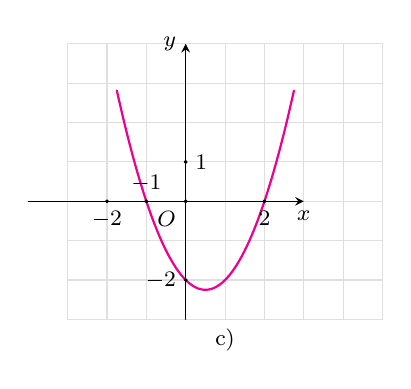
\begin{tikzpicture}[scale=.5, font=\footnotesize, line join=round, line cap=round, >=stealth]
		\draw[gray!50,opacity=.5](-3,-3)grid(5,4);
		\draw[->](-4,0)--(0,0)node[below left]{$O$}--(3,0)node[below]{$x$};
		\draw[->](0,-3)--(0,4)node[left]{$y$};
		\draw[smooth,domain=-1.75:2.75,thick,magenta]plot(\x,{(\x)^2-(\x)-2});
		\draw (1,-3)node[below]{c)};
		\draw(0,1)node[right]{$1$};
		\draw(0,-2)node[left]{$-2$};
		\draw(-2,0)node[below]{$-2$};
		\draw(-1,0)node[above]{$-1$};
		\draw(2,0)node[below]{$2$};
		\foreach \x in {-2,-1,0,2}\draw[fill](\x,0)circle(1pt);
		\foreach \x in {-2,1}\draw[fill](0,\x)circle(1pt);
		
	\end{tikzpicture}
	\loigiai{
		\begin{enumEX}[a)]{1}
			\item \immini{Từ đồ thị hình a) ta có nghiệm của tam thức bậc hai $f(x)$ là $x=2$. Bảng xét dấu của tam thức là}{
				
\begin{tikzpicture}
					\tkzTabInit[deltacl=0.6,espcl=2.5,lgt=2,nocadre=false]
					{$x$/0.6,$f(x)$/0.6}
					{$-\infty$,$2$,$+\infty$}
					\tkzTabLine{,+,0,+,}
					
				\end{tikzpicture}
			}
			\item \immini{Từ đồ thị hình b) ta có tam thức bậc hai $f(x)$ có $2$ nghiệm $x_1=-4$ và $x_2=-1$. Bảng xét dấu của tam thức là}{
				
\begin{tikzpicture}
					\tkzTabInit[deltacl=0.6,espcl=2.5,lgt=2,nocadre=false]
					{$x$/0.6,$f(x)$/0.6}
					{$-\infty$,$-4$,$-1$,$+\infty$}
					\tkzTabLine{,-,0,+,0,-,}
					
				\end{tikzpicture}
			}
			\item \immini{Từ đồ thị hình c) ta có nghiệm của tam thức bậc hai $f(x)$ là $x_1=-1$ và $x_2=2$. Bảng xét dấu của tam thức là}{
				
\begin{tikzpicture}
					\tkzTabInit[deltacl=0.6,espcl=2.5,lgt=2,nocadre=false]
					{$x$/0.6,$f(x)$/0.6}
					{$-\infty$,$-1$,$2$,$+\infty$}
					\tkzTabLine{,+,0,-,0,+,}
					
				\end{tikzpicture}
			}
		\end{enumEX}
	}
\end{vd}

\begin{dang}{Giải bất phương trình bậc hai}
	Ta lập bảng xét dấu của tam thức bậc hai. Sau đó, chọn  kết quả phù hợp với yêu cầu đề bài.
\end{dang}
\begin{vd}%[0D4Y5-2]
	Giải các bất phương trình sau	
	\begin{listEX}[3]
		\item $-3x^2+2x+1<0$.
		\item $x^2+x-12\ge 0$.
		\item $-x^2+x+6 \le 0$.
		\item $-x^2+x-5<0$
		\item $x^2-2x-4>0$
		\item $4x^2+4x+1>0$
	\end{listEX}
	\loigiai{
		\begin{listEX}
			\item Ta có $-3x^2+2x+1=0 \Leftrightarrow x=-\dfrac{1}{3}$ hoặc $x=1$.\\
			Bảng xét dấu
			\begin{center}
				\begin{tikzpicture}
					\tkzTabInit[lgt=3,espcl=2]
					{$x$ /1.2, $-x^2+4x+5$ /0.8}
					{$-\infty$,$-\dfrac{1}{3}$,$1$,$+\infty$}
					\tkzTabLine{ ,-,$0$,+,$0$,-,}
				\end{tikzpicture}
			\end{center}
			Dựa vào bảng xét dấu, ta có tập nghiệm của bất phương trình là $S=\left(-\infty;-\dfrac{1}{3}\right)\cup (1;+\infty)$.
			\item Ta có $x^2+x-12=0 \Leftrightarrow x=3$ hoặc $x=-4$.\\
			Bảng xét dấu
			\begin{center}
				
\begin{tikzpicture}
					\tkzTabInit[lgt=3,espcl=2]
					{$x$ /0.8, $x^2+x-12$/0.8}
					{$-\infty$,$-4$,$3$,$+\infty$}
					\tkzTabLine{ ,+,$0$,-,$0$,+,}
				\end{tikzpicture}
			\end{center}
			Dựa vào bảng xét dấu, ta có tập nghiệm của bất phương trình là $S=(-\infty;-4] \cup [3;+\infty)$.	
			\item Ta có $-x^2+x+6=0 \Leftrightarrow x=-2$ hoặc $x=3$.
			Bảng xét dấu
			\begin{center}
				\begin{tikzpicture}
					\tkzTabInit[lgt=3,espcl=2]
					{$x$ /1.2, $-x^2+x+6$ /0.8}
					{$-\infty$,$-2$,$3$,$+\infty$}
					\tkzTabLine{ ,-,$0$,+,$0$,-,}
				\end{tikzpicture}
			\end{center}
			Dựa vào bảng xét dấu, ta có tập nghiệm của bất phương trình là $S=\left(-\infty;-2\right]\cup [3;+\infty)$.
			\item $-x^2+x-5=0$ vô nghiệm nên ta có bảng xét dấu
			\begin{center}
				\begin{tikzpicture}
					\tkzTabInit[lgt=3,espcl=2]
					{$x$ /0.8, $-x^2+x-5$ /0.8}
					{$-\infty$,$+\infty$}
					\tkzTabLine{ ,-,}
				\end{tikzpicture}
			\end{center}
			Dựa vào bảng xét dấu, ta có tập nghiệm của bất phương trình là $\mathbb{R}$.
			\item Ta có $x^2-2x-4>0\Leftrightarrow x\in\left(-\infty;1-\sqrt{5}\right)\cup \left(1+\sqrt{5};+\infty\right)$.
			\item Ta có $4x^2+4x+1=0\Leftrightarrow x=-\dfrac{1}{2} $.\\
			Bảng xét dấu
			\begin{center}
				
\begin{tikzpicture}
					\tkzTabInit[lgt=3,espcl=2]
					{$x$ /1.2, $4x^2+4x+1$ /0.8}
					{$-\infty$,$-\frac{1}{2}$,$+\infty$}
					\tkzTabLine{ ,+,$0$,+,}
				\end{tikzpicture}
			\end{center}
			Tập nghiệm của bất phương trình là $\mathbb{R}\setminus\left\{-\dfrac{1}{2}\right\}$.
			
		\end{listEX}
	}
\end{vd}
\begin{vd}
	Tìm nghiệm của bất phương trình $ax^2+bx+c>0$, với đồ thị $f(x)=ax^2+bx+c$ được cho ở mỗi hình bên:\\
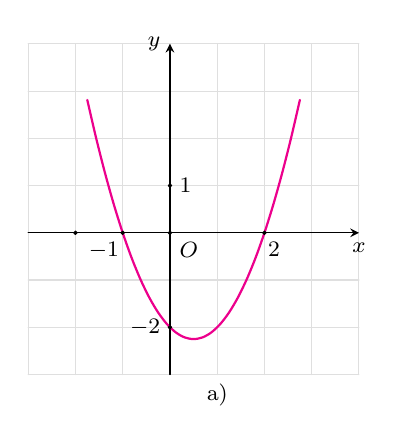
\begin{tikzpicture}[scale=.6, font=\footnotesize, line join=round, line cap=round, >=stealth]
	\draw[gray!50,opacity=.5](-3,-3)grid(4,4);
	\draw[->](-3,0)--(0,0)node[below right]{$O$}--(4,0)node[below]{$x$};
	\draw[->](0,-3)--(0,4)node[left]{$y$};
	\draw[smooth,domain=-1.75:2.75,thick, magenta]plot(\x,{(\x)^2-(\x)-2});
	\draw (1,-3)node[below]{a)};
	\draw(0,1)node[right]{$1$};
	\draw(0,-2)node[left]{$-2$};
	\draw(-1.4,0)node[below]{$-1$};
	\draw(2.2,0)node[below]{$2$};
	\foreach \x in {-2,-1,0,2}\draw[fill](\x,0)circle(1pt);
	\foreach \x in {-2,1}\draw[fill](0,\x)circle(1pt);
\end{tikzpicture}\hspace{1cm}
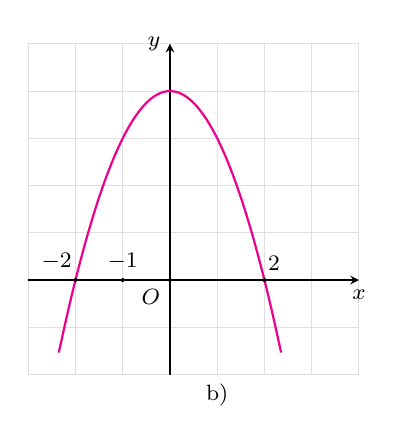
\begin{tikzpicture}[scale=.6, font=\footnotesize, line join=round, line cap=round, >=stealth]
	\draw[gray!50,opacity=.5](-3,-2)grid(4,5);
	\draw[->](-3,0)--(0,0)node[below left]{$O$}--(4,0)node[below]{$x$};
	\draw[->](0,-2)--(0,5)node[left]{$y$};
	\draw[smooth,domain=-2.35:2.35,thick, magenta]plot(\x,{-(\x)^2+4});
	\draw (1,-2)node[below]{b)};
	\draw(-2.4,0)node[above]{$-2$};
	\draw(-1,0)node[above]{$-1$};
	\draw(2.2,0)node[above]{$2$};
	\foreach \x in {-2,-1,0,2}\draw[fill](\x,0)circle(1pt);
\end{tikzpicture}\hspace{1cm}
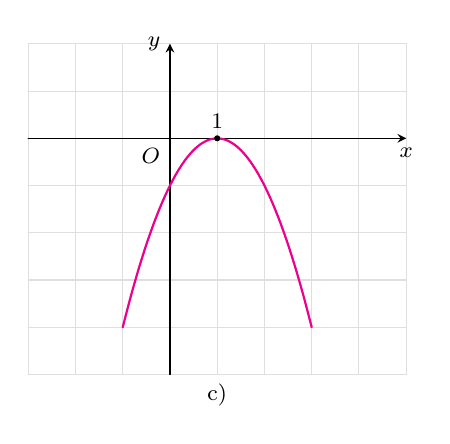
\begin{tikzpicture}[scale=.6, font=\footnotesize, line join=round, line cap=round, >=stealth]
	\draw[gray!50,opacity=.5](-3,-5)grid(5,2);
	\draw[->](-3,0)--(0,0)node[below left]{$O$}--(5,0)node[below]{$x$};
	\draw[->](0,-5)--(0,2)node[left]{$y$};
	\draw[smooth,domain=-1:3,thick, magenta]plot(\x,{-(\x-1)^2});
	\draw (1,-5)node[below]{c)};
	\draw(1,0)node[above]{$1$};
	\foreach \x in {1}\draw[fill](\x,0)circle(1.5pt);
\end{tikzpicture}
	\loigiai{}
\end{vd}
\begin{dang}{Vận dụng, thực tiễn}
\end{dang}

\begin{vd}
	Tìm các giá trị của tham số $m$ để 
	\begin{enumEX}[a)]{2}
		\item $x^2 - 2x + m \geq 0,\, \forall x\in  \mathbb{R}$.
		\item $x^2 -2mx + 4- 3m>0,\, \forall x\in  \mathbb{R} $. 
		\item $-x^2 -2 (2m-1) x+ 1 -2m \le 0,\, \forall x\in  \mathbb{R} $. 
		\item $-2x^2+2(m-2)x+m-2<0,\, \forall x\in  \mathbb{R} $. 
	\end{enumEX}
	\loigiai{
		\begin{itemize}
			\item [a)] Bất phương trình thỏa mãn với mọi số thực thì $\Delta \leq 0 \ (\Delta' \leq 0)$.\\
			$\Delta' = (-1)^2 - m \leq 0 \Leftrightarrow m \geq 1$.
			\item [b)] Ta có $\Delta '= b'^2 -a c = m^2 + 3m-4$.\\
			Khi đó $P(x) >0 $ $\forall x \Leftrightarrow \heva{& a > 0\\& \Delta ' <0 } \Leftrightarrow \heva{& 1 >0 \text{ (luôn đúng)}\\& m^2 + 3m -4 < 0} \Leftrightarrow m^2 + 3m -4 <0$.\\
			Bảng xét dấu \\
			\begin{center}
				
\begin{tikzpicture}
					\tkzTabInit
					[lgt=2.5,espcl=2] % tùy chọn
					{$m $/1, $m^2 + 3m -4 $/1.3} % cột 1
					{$-\infty $,$-4$,$1$,$+ \infty $} % hàng 1 cột 2
					\tkzTabLine{, +  , z , - , z , + , } % hàng 2 cột 2
				\end{tikzpicture}
			\end{center}
			Dựa vào bảng xét dấu ta thấy $m \in (-4;1)$ thoả mãn yêu cầu bài toán.
			\item [c)] Ta có $\Delta ' = b'^2 - ac = (2m-1)^2 + (1-2m) = 4m^2 -6m +2. $\\
			Khi đó $P(x) \le 0$ $\forall x \Leftrightarrow \heva{&a <0 \\& \Delta ' \le 0} \Leftrightarrow \heva{&-1<0 \text{ (luôn đúng)} \\& 4m^2 - 6m+2 \le 0} \Leftrightarrow 4m^2 - 6m+2 \le 0. $\\
			Bảng xét dấu \\
			\begin{center}
				
\begin{tikzpicture}
					\tkzTabInit
					[lgt=3 ,espcl=2] % tùy chọn
					{$m$/1, $4m^2 -6m +2  $/1.3} % cột 1
					{$-\infty $,$\dfrac{1}{2}$,$1$,$+ \infty $} % hàng 1 cột 2
					\tkzTabLine{, +  , z , - , z , + , } % hàng 2 cột 2
				\end{tikzpicture}
			\end{center}
			Dựa vào bảng xét dấu ta thấy $m \in \left[ \dfrac{1}{2};1\right]$ thoả mãn yêu cầu bài toán.
			\item [d)] Yêu cầu bài toán tương đương với
			{\allowdisplaybreaks
				\begin{eqnarray*}
					&&f(x)=-2x^2+2(m-2)x+m-2\le 0,\forall x\in\mathbb{R} \\
					&\Leftrightarrow & \Delta' =(m-2)^2+2\cdot(m-2)< 0\\
					&\Leftrightarrow & m(m-2)< 0\\
					&\Leftrightarrow & 0< m< 2.
			\end{eqnarray*}}
			Vậy, giá trị cần tìm của $m$ là $0< m< 2$.
		\end{itemize}
	}
\end{vd}

\begin{vd}
	Độ cao so với mặt đất của một quả bóng được ném lên theo phương thẳng đứng được mô tả bởi hàm số bậc hai $h(t)=-4,9 t^{2}+20 t+1$, ở đó độ cao $h(t)$ tính bằng mét và thời gian $t$ tính bằng giây. Trong khoảng thời điểm nào trong quá trình bay của nó, quả bóng sẽ ở độ cao trên $5$ m so với mặt đất?
	\loigiai{
		Xét bất phương trình $$-4,9 t^{2}+20 t+1>5\Leftrightarrow-4,9 t^{2}+20 t-4>0$$
		Nghiệm của phương trình
		$-4,9 t^{2}+20 t-4=0$ là $t \approx 0,21 ; t \approx 3,87$.
		Do đó, nghiệm của bất phương trình là $t \in(0,21 ; 3,87)$. Vậy khoảng thời điểm $t \in(0,21 ; 3,87)$
		(s) trong quá trình bay của quả bóng thì nó sẽ ở độ cao trên $5 \mathrm{~m}$ so với mặt đất.}
\end{vd}

\begin{vd}
	Một vật được ném theo phương thẳng đứng xuống dưới từ độ cao $320 \mathrm{~m}$ với vận tốc ban đầu $v_{Q}=20 \mathrm{~m} / \mathrm{s}$. Hỏi sau ít nhất bao nhiêu giây, vật đó cách mặt đất không quá $100 \mathrm{~m}$ ? Giả thiết rằng sức cản của không khí là không đáng kể.
	\loigiai{
		Độ cao của vật so với mặt đất được cho bởi công thức
		$$
		h(t)=h_{0}+v_{0} t-\frac{1}{2} g t^{2}=320+20 t-4,9 t^{2}(\mathrm{~m}) .
		$$
		Vật cách mặt đất không quá $100 \mathrm{~m}$ khi và chỉ khi $h(t) \leq 100$, tức là $-4,9 t^{2}+20 t+320 \leq 100$ hay tương đương $4,9 t^{2}-20 t-220 \geq 0$.\\
		Giải bất phương trình này và chú ý đến điều kiện $t>0$ ta được: $t \geq \frac{10+\sqrt{1178}}{4,9} \approx 9,05(\mathrm{~s})$.
	}
\end{vd}

\begin{vd}
	\immini{Xét đường tròn đường kính $AB=4$ và một điểm $M$ di chuyển trên đoạn $A B$, đặt $A M=x$. Xét hai đường tròn đường kính $A M$ và $M B$. Kí hiệu $S(x)$ là diện tích phần hình phẳng nằm trong hình tròn lớn và nằm ngoài hai hình tròn nhỏ. Xác định các giá trị của $x$ để diện tích $S(x)$ không vượt quá một nửa tổng diện tích hai hình tròn nhỏ.}{
		\begin{tikzpicture}[smooth,font=\footnotesize,scale=1,>=latex]
			\path
			(0,0) coordinate (A)
			(4,0) coordinate (B)
			(1.5,0) coordinate (M)
			($(A)!0.5!(B)$)coordinate (O)
			($(A)!0.5!(M)$)coordinate (O1)
			($(M)!0.5!(B)$)coordinate (O2)
			($(A)+(0,3)$)coordinate (X)
			($(A)+(0,2.3)$)coordinate (X')
			($(B)+(0,3)$)coordinate (Y)
			($(M)+(0,2.3)$)coordinate (Y')
			;
			\fill[cyan] (O) circle (2);
			\fill[white] (O1) circle (0.75);
			\fill[white] (O2) circle (1.25);
			\draw 
			(O) circle (2)
			(O1) circle (0.75)
			(O2) circle (1.25);
			\draw[dashed,<->](X)--(Y)node[above,midway,sloped,scale=.8]{$4$ };
			\draw[dashed,<->](X')--(Y')node[above,midway,sloped,scale=.8]{$x$ };
			\draw[dashed](A)--(X) (B)--(Y) (M)--(Y');
			\draw(A)node[left]{$A$}--(M)node[below right]{$M$}--(B)node[right]{$B$};
			%\path (A)--(M1) node[below,midway,sloped,scale=.8]{\scriptsize $3,2$m }
	\end{tikzpicture}}
	\loigiai{
		Vì điểm $M$ nằm giữa $A$ và $B$ nên $M B=A B-A M=4-x$.
		Gọi $S, S_{1}, S_{2}$ lần lượt là diện tích hình tròn đường kính $A B, A M$ và $M B$.
		Ta có: $\quad S_{1}+S_{2}=\pi\left(\frac{x}{2}\right)^{2}+\pi\left(\frac{4-x}{2}\right)^{2}=\frac{x^{2}-4 x+8}{2} \pi$.
		$$
		S(x)=S-\left(S_{1}+S_{2}\right)=4 \pi-\frac{x^{2}-4 x+8}{2} \pi=\frac{-x^{2}+4 x}{2} \pi .
		$$
		Do đó từ điều kiện $S(x) \leq \frac{1}{2}\left(S_{1}+S_{2}\right)$ ta được bất phương trình bậc hai $3 x^{2}-12 x+8 \geq 0$.
		Giải bất phương trình bậc hai này và kết hợp với điều kiện $0 \leq x \leq 4$, ta được
		$$
		x \in\left[0 ; \frac{6-2 \sqrt{3}}{3}\right] \cup\left[\frac{6+2 \sqrt{3}}{3} ; 4\right]
		$$}
\end{vd}

\begin{vd}%[0D4K5-1]
	Để xây dựng phương án kinh doanh cho một loại sản phẩm, doanh nghiệp tính toán lợi nhuận $y$ (đồng) theo công thức sau $y=-200x^2+92000x-8400000$, trong đó $x$ là số sản phẩm được bán ra. Cho biết doanh nghiệp có lãi khi nào, bị lỗ khi nào.
	\loigiai{
		Xét tam thức bậc hai $f(x)=-200x^2+92000x-8400000$.\\
		$f(x)$ có hai nghiệm là $x_1=\dfrac{-460+\sqrt{43600}}{-2}\approx125{,}6$ và $x_2=\dfrac{-460-\sqrt{43600}}{-2}\approx334{,}4$ và hệ số $a=-200<0$. Ta có bảng xét dấu như sau
		\begin{center}
			
\begin{tikzpicture}
				\tkzTabInit[deltacl=0.6,espcl=2.5,lgt=2,nocadre=false]
				{$x$/0.6,$f(x)$/0.6}
				{$-\infty$,$x_1$,$x_2$,$+\infty$}
				\tkzTabLine{,-,0,+,0,-,}
				
			\end{tikzpicture}
		\end{center}
		Vì $x$ là số nguyên dương nên:
		\begin{itemize}
			\item Doanh nghiệp có lãi khi và chỉ khi $f(x)>0$, tức là $126\le x\le334$.
			\item Doanh nghiệp bị lỗ khi và chỉ khi $f(x)<0$, tức là $x\le125$ hoặc $x\ge335$.
		\end{itemize}
		Vậy doanh nghiệp có lãi khi bán từ $126$ đến $334$ sản phẩm, doanh nghiệp bị lỗ khi bán tối đa $125$ sản phẩm hoặc bán tối thiểu $335$ sản phẩm.
	}
\end{vd}

\begin{vd}%
	\immini{Một tình huống trong huấn luyện pháo binh được mô tả như sau: Trong mặt phẳng tọa độ $Oxy$, khẩu đại bác được biểu thị bằng điểm $O(0; 0)$ và bia mục tiêu được biểu thị bằng đoạn thẳng $MN$ với $M(2100; 25)$ và $N(2100; 15)$ (Hình 29). Xạ thủ cần xác định parabol $y=-a^2x^2+10ax$ $(a>0)$ mô tả quỹ đạo chuyển động của viên đạn sao cho viên đạn bắn ra từ khẩu đại bác phải chạm vào bia mục tiêu. Tìm giá trị lớn nhất của $a$ để xạ thủ đạt được mục đích trên.
	}{\begin{tikzpicture}[scale=1, font=\footnotesize, line join=round, line cap=round, >=stealth]
			\def\a{-.25} \def\b{1} \def\c{0} % Hệ số
			\def\xt{-1} \def\xp{6} \def\yt{3} \def\yd{-1} % x_trái, x_phải, y_trên, y_dưới (giới hạn)
			\draw[->] (\xt,0)--(\xp,0) node [below]{$x$};
			\draw[->] (0,\yd)--(0,\yt) node [left]{$y$};
			\node at (0,0) [below left]{$O$};
			\clip (\xt-0.1,\yd+0.1) rectangle (\xp-0.1,\yt-0.1);
			\draw[smooth,samples=300,domain=0:4] plot(\x,{\a*(\x)^2+\b*(\x)+\c});
			\draw[fill=black] (3,0) node[shift={(-90:.4)}]{$2100$} circle(1pt);
			\draw[fill=black] (3,1) node[shift={(90:.4)}]{$M$} circle(1pt);
			\draw[fill=black] (3,.5) node[shift={(180:.3)}]{$N$} circle(1pt);
			\draw[line width=2pt] (3,1)--(3,.5);
			\draw (2,1) node[shift={(90:1)}]{$y=-a^2x^2+10ax$};
			\draw (2,-1) node[shift={(-90:.4)}]{Hình 29};
			
	\end{tikzpicture}}
	\loigiai
	{
		Tại vị trí $x=2100$, độ cao của viên đạn là
		\[y=-a^2\cdot 2100^2+10a\cdot 2100=-4410000a^2+21000a.\]
		Viên đạn chạm được vào bia mục tiêu khi và chỉ khi $a$ thoả mãn các bất phương trình sau
		\allowdisplaybreaks
		\begin{align*}
			&2100\leq\dfrac{10}{a} \tag{5}; \\
			&-4410000a^2+21000a\leq 25  \tag{6};\\
			&-4410000a^2+21000a\geq 15  \tag{7}.
		\end{align*}
		\begin{itemize}
			\item $(5)\Leftrightarrow\dfrac{1}{a}\geq 210\Leftrightarrow a\leq\dfrac{1}{210}$. Vì $a>0$ nên $a\in\left(0;\dfrac{1}{210}\right]$.
			\item $(6) \Leftrightarrow 4410000a^2-21000a+25\geq 0 \Leftrightarrow(2100a-5)^2\geq 0$. Bất phương trình này đúng $\forall a>0$.
			\item \allowdisplaybreaks
			$\begin{aligned}[t]
				(7)&\Leftrightarrow 4410000a^2-21000a+15\leq 0\Leftrightarrow\dfrac{1}{420}-\dfrac{\sqrt{10}}{2100}\leq a\leq\dfrac{1}{420}+\dfrac{\sqrt{10}}{2100}\\
				&\Leftrightarrow a\in\left[\dfrac{1}{420}-\dfrac{\sqrt{10}}{2100};\dfrac{1}{420}+\dfrac{\sqrt{10}}{2100}\right].
			\end{aligned}$
		\end{itemize}
		Do $\dfrac{1}{420}-\dfrac{\sqrt{10}}{2100}>0$ và $\dfrac{1}{420}+\dfrac{\sqrt{10}}{2100}<\dfrac{1}{210}$ nên
		\[\left(0;\dfrac{1}{210}\right]\cap\left[\dfrac{1}{420}-\dfrac{\sqrt{10}}{2100};\dfrac{1}{420}+\dfrac{\sqrt{10}}{2100}\right]=\left[\dfrac{1}{420}-\dfrac{\sqrt{10}}{2100};\dfrac{1}{420}+\dfrac{\sqrt{10}}{2100}\right].\]
		Vì thế, viên đạn chạm được vào bia mục tiêu khi và chỉ khi
		\[a\in\left[\dfrac{1}{420}-\dfrac{\sqrt{10}}{2100};\dfrac{1}{420}+\dfrac{\sqrt{10}}{2100}\right].\]
		Vậy giá trị lớn nhất của $a$ là $\dfrac{1}{420}+\dfrac{\sqrt{10}}{2100}$.
	}
\end{vd}


\subsection{BÀI TẬP TỰ LUYỆN}

\begin{bt}%[0D4Y5-1]
	Xét dấu của mỗi tam thức bậc hai sau
	\begin{enumEX}[a)]{3}
		\item $f(x)=3x^2-4x+1$;
		\item $f(x)=9x^2+6x+1$;
		\item $f(x)=2x^2-3x+10$;
		\item $f(x)=-5x^2+2x+3$;
		\item $f(x)=-4x^2+8x-4$;
		\item $f(x)=-3x^2+3x-1$.
	\end{enumEX}
	\loigiai{
		\begin{enumEX}[a)]{1}
			\item $f(x)=3x^2-4x+1$ có $2$ nghiệm $x_1=1$ và $x_2=\dfrac{1}{3}$.\\
			Bảng xét dấu
			\begin{center}
				
\begin{tikzpicture}
					\tkzTabInit[deltacl=0.6,espcl=2.5,lgt=2,nocadre=false]
					{$x$/0.6,$f(x)$/0.6}
					{$-\infty$,$\tfrac{1}{3}$,$1$,$+\infty$}
					\tkzTabLine{,+,0,-,0,+,}
					
				\end{tikzpicture}
			\end{center}
			\begin{itemize}
				\item $f(x)>0$ khi và chỉ khi $x\in\left(-\infty;\dfrac{1}{3}\right)\cup(1;+\infty)$.
				\item $f(x)<0$ khi và chỉ khi $x\in\left(\dfrac{1}{3};1\right)$.
			\end{itemize}
			\item $f(x)=9x^2+6x+1$ có nghiệm kép $x=-\dfrac{1}{3}$.\\
			Bảng xét dấu
			\begin{center}
				
\begin{tikzpicture}
					\tkzTabInit[deltacl=0.6,espcl=2.5,lgt=2,nocadre=false]
					{$x$/0.6,$f(x)$/0.6}
					{$-\infty$,$-\tfrac{1}{3}$,$+\infty$}
					\tkzTabLine{,+,0,+,}
					
				\end{tikzpicture}
			\end{center}
			$f(x)>0$ khi và chỉ khi $x\in\mathbb{R}\setminus\left\{-\dfrac{1}{3}\right\}$.
			\item $f(x)=2x^2-3x+10$ vô nghiệm vì $\Delta=-71<0$ và $a=2>0$.\\
			Do đó $f(x)>0$ với mọi $x\in\mathbb{R}$.
			\item $f(x)=-5x^2+2x+3$ có $2$ nghiệm $x_1=1$ và $x_2=-\dfrac{3}{5}$.\\
			Bảng xét dấu
			\begin{center}
				
\begin{tikzpicture}
					\tkzTabInit[deltacl=0.6,espcl=2.5,lgt=2,nocadre=false]
					{$x$/0.6,$f(x)$/0.6}
					{$-\infty$,$-\tfrac{3}{5}$,$1$,$+\infty$}
					\tkzTabLine{,-,0,+,0,-,}
					
				\end{tikzpicture}
			\end{center}
			\begin{itemize}
				\item $f(x)<0$ khi và chỉ khi $x\in\left(-\infty;-\dfrac{3}{5}\right)\cup(1;+\infty)$.
				\item $f(x)>0$ khi và chỉ khi $x\in\left(-\dfrac{3}{5};1\right)$.
			\end{itemize}
			\item $f(x)=-4x^2+8x-4$ có nghiệm kép $x=1$.\\
			Bảng xét dấu
			\begin{center}
				
\begin{tikzpicture}
					\tkzTabInit[deltacl=0.6,espcl=2.5,lgt=2,nocadre=false]
					{$x$/0.6,$f(x)$/0.6}
					{$-\infty$,$1$,$+\infty$}
					\tkzTabLine{,-,0,-,}
					
				\end{tikzpicture}
			\end{center}
			$f(x)<0$ khi và chỉ khi $x\in\mathbb{R}\setminus\left\{1\right\}$.
			\item $f(x)=-3x^2+3x-1$ vô nghiệm vì $\Delta=-3<0$ và $a=-3<0$.\\
			Do đó $f(x)<0$ với mọi $x\in\mathbb{R}$.
		\end{enumEX}
	}
\end{bt}

\begin{bt}%[0D4B5-1]
	Tìm nghiệm và lập bảng xét dấu của tam thức bậc hai $f(x)$ ứng với đồ thị hàm số $y=f(x)$ được cho ở mỗi hình sau.\\
	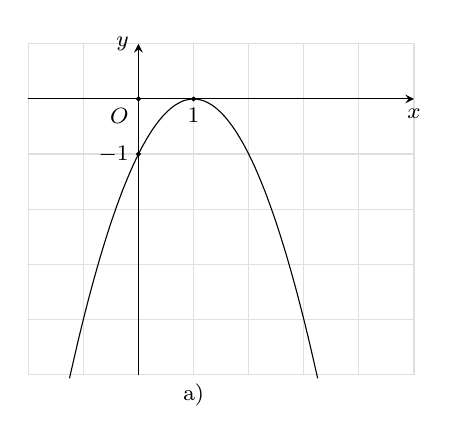
\begin{tikzpicture}[scale=.7, font=\footnotesize, line join=round, line cap=round, >=stealth]
		\draw[gray!50,opacity=.5](-2,-5)grid(5,1);
		\draw[->](-2,0)--(0,0)node[below left]{$O$}--(5,0)node[below]{$x$};
		\draw[->](0,-5)--(0,1)node[left]{$y$};
		\draw[smooth,domain=-1.25:3.25]plot(\x,{-(\x)^2+2*(\x)-1});
		\draw (1,-5)node[below]{a)};
		\draw(1,0)node[below]{$1$};
		\draw(0,-1)node[left]{$-1$};
		\foreach \x in{0,1}\draw[fill](\x,0)circle(1pt);
		\draw[fill](0,-1)circle(1pt);
	\end{tikzpicture}\hspace*{1cm}
	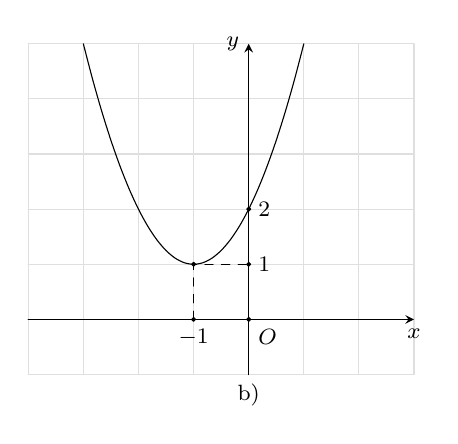
\begin{tikzpicture}[scale=.7, font=\footnotesize, line join=round, line cap=round, >=stealth]
		\draw[gray!50,opacity=.5](-4,-1)grid(3,5);
		\draw[->](-4,0)--(0,0)node[below right]{$O$}--(3,0)node[below]{$x$};
		\draw[->](0,-1)--(0,5)node[left]{$y$};
		\draw[smooth,domain=-3:1]plot(\x,{(\x)^2+2*(\x)+2});
		\draw (0,-1)node[below]{b)};
		\draw(0,1)node[right]{$1$};
		\draw(0,2)node[right]{$2$};
		\draw(-1,0)node[below]{$-1$};
		\draw[dashed](-1,0)--(-1,1)--(0,1);
		\foreach \x in {0,1,2}\draw[fill](0,\x)circle(1pt);
		\draw[fill](-1,0)circle(1pt);
		\draw[fill](-1,1)circle(1pt);
		
	\end{tikzpicture}\hspace*{1cm}
	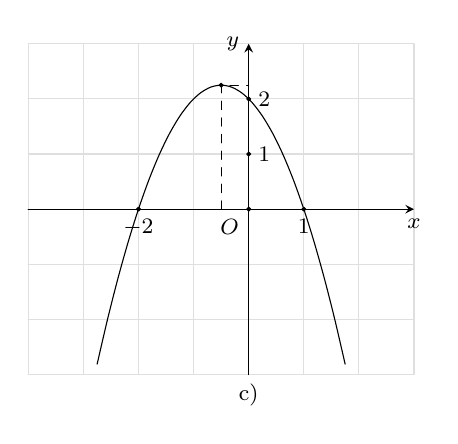
\begin{tikzpicture}[scale=.7, font=\footnotesize, line join=round, line cap=round, >=stealth]
		\draw[gray!50,opacity=.5](-4,-3)grid(3,3);
		\draw[->](-4,0)--(0,0)node[below left]{$O$}--(3,0)node[below]{$x$};
		\draw[->](0,-3)--(0,3)node[left]{$y$};
		\draw[smooth,domain=-2.75:1.75]plot(\x,{-(\x)^2-(\x)+2});
		\draw (0,-3)node[below]{c)};
		\draw(0,1)node[right]{$1$};
		\draw(0,2)node[right]{$2$};
		\draw(-2,0)node[below]{$-2$};
		\draw(1,0)node[below]{$1$};
		\draw[dashed](-0.5,0)--(-1/2,2.25)--(0,2.25);
		\foreach \x in {-2,0,1}\draw[fill](\x,0)circle(1pt);
		\foreach \x in {1,2}\draw[fill](0,\x)circle(1pt);
		\draw[fill](-1/2,2.25)circle(1pt);
		
	\end{tikzpicture}
	\loigiai{
		\begin{enumEX}[a)]{1}
			\item \immini{Từ đồ thị hình a) ta có nghiệm của tam thức bậc hai $f(x)$ là $x=1$. Bảng xét dấu của tam thức là}{
				
\begin{tikzpicture}
					\tkzTabInit[deltacl=0.6,espcl=2.5,lgt=2,nocadre=false]
					{$x$/0.6,$f(x)$/0.6}
					{$-\infty$,$1$,$+\infty$}
					\tkzTabLine{,-,0,-,}
					
				\end{tikzpicture}
			}
			\item \immini{Từ đồ thị hình b) ta có tam thức bậc hai $f(x)$ vô nghiệm. Bảng xét dấu của tam thức là}{
				
\begin{tikzpicture}
					\tkzTabInit[deltacl=0.6,espcl=2.5,lgt=2,nocadre=false]
					{$x$/0.6,$f(x)$/0.6}
					{$-\infty$,,$+\infty$}
					\tkzTabLine{,,+,}
					
				\end{tikzpicture}
			}
			\item \immini{Từ đồ thị hình c) ta có nghiệm của tam thức bậc hai $f(x)$ là $x_1=-2$ và $x_2=1$. Bảng xét dấu của tam thức là}{
				
\begin{tikzpicture}
					\tkzTabInit[deltacl=0.6,espcl=2.5,lgt=2,nocadre=false]
					{$x$/0.6,$f(x)$/0.6}
					{$-\infty$,$-2$,$1$,$+\infty$}
					\tkzTabLine{,-,0,+,0,-,}
					
				\end{tikzpicture}
			}
		\end{enumEX}
	}
\end{bt}

\begin{bt}
	Giải các bất phương trình sau:
	\begin{enumEX}[a)]{2}
		\item  $x^2-3x+2<0$ 
		\item  $6x^2+x-1\le 0$
		\item $-9x^2 + 6x -1>0$.
		\item $12-x-x^2\ge 0$.
	\end{enumEX}
\loigiai{
\begin{enumerate}[a)]
	\item Đặt $f(x)=x^2-3x+2$ và $f(x)=0\Leftrightarrow x^2-3x+2=0\Leftrightarrow\hoac{&x=2\\&x=1.}$\\
	Bảng xét dấu
	\begin{center}
		
\begin{tikzpicture}[>=stealth]
			\tkzTabInit[nocadre=false,lgt=1.2,espcl=2,deltacl=1]{$x$/.7 ,$f(x)$/.7}
			{$-\infty$ , $1$ , $2$ , $+\infty$}
			\tkzTabLine{ ,+ , $0$ , - , $0$ , + , }
		\end{tikzpicture}
	\end{center}
	Dựa vào bảng xét dấu, tập nghiệm của bất phương trình đã cho là
	\[S=(1;2).\]
	\item Bảng xét dấu
	\begin{center}
		
\begin{tikzpicture}[>=stealth]
			\tkzTabInit[nocadre=false,lgt=3,espcl=2,deltacl=1]{$x$/1 ,$6x^2+x-1$/.7}
			{$-\infty$ , $-\dfrac{1}{2}$ , $\dfrac{1}{3}$ , $+\infty$}
			\tkzTabLine{ ,+ , $0$ , - , $0$ ,+ , }
		\end{tikzpicture}
	\end{center}
	Từ bảng xét dấu, ta có tập nghiệm của bất phương trình là
	\[S=\left[-\dfrac{1}{2};\dfrac{1}{3}\right].\]
	\item Cho $-9x^2 + 6x -1=0 \Leftrightarrow x = \dfrac{1}{3}$.
	Bảng xét dấu
	\begin{center}
		\begin{tikzpicture}
			\tkzTabInit
			[lgt=2.8,espcl=2] % tùy chọn
			{$x$/1, $-9x^2 + 6x -1 $/1.5} % cột 1
			{$-\infty $, $\dfrac{1}{3}$ ,$+ \infty $} % hàng 1 cột 2
			\tkzTabLine{, -, z , -, } % hàng 2 cột 2
		\end{tikzpicture}
	\end{center}
	Vậy $S= \emptyset$.
	\item Cho $-x^2 -x+12=0 \Leftrightarrow \hoac{&x =-4 \\& x=3.}$\\
	Bảng xét dấu
	\begin{center}
		\begin{tikzpicture}
			\tkzTabInit
			[lgt=2.5,espcl=2] % tùy chọn
			{$x$/1, $-x^2 -x+12 $/1.5} % cột 1
			{$-\infty $, $-4$,$3$ ,$+ \infty $} % hàng 1 cột 2
			\tkzTabLine{, - , z , + , z , -, } % hàng 2 cột 2
		\end{tikzpicture}
	\end{center}
	Vậy $S= [-4;3]$.
\end{enumerate}}
\end{bt}
\begin{bt}%[0D4B5-2]
	Tìm tất cả giá trị thực của tham số $m$ để
	\begin{enumEX}[a)]{1}
		\item phương trình $2x^2+2\left( m+2 \right)x+3+4m+{m^2}=0$ có nghiệm.
		\item phương trình $x^2-(m+1)x+1=0$ vô nghiệm.
		\item phương trình $x^2+2(m+1)x+9m-5=0$ có hai nghiệm phân biêt.
	\end{enumEX}
	\loigiai
	{
		\begin{enumerate}[a)]
			\item Phương trình $2x^2+2(m+2)x+3+4m+m^2=0$ có $\Delta'=(m+2)^2-2(m^2+4m+3) = -m^2-4m-2$.\\
			Yêu cầu bài toán thỏa mãn khi
			\allowdisplaybreaks
			\begin{eqnarray*}
				\Delta' \geq 0 &\Leftrightarrow & -m^2-4m-2 \geq 0\\
				&\Leftrightarrow & -2-\sqrt{2} \leq m \leq -2+\sqrt{2}.
			\end{eqnarray*}
			Vậy với $m \in \left[-2-\sqrt{2};-2+\sqrt{2}\right]$ thì phương trình đã cho có nghiệm.
			\item Phương trình vô nghiệm khi và chỉ khi
			\begin{eqnarray*}
				\Delta <0 \Leftrightarrow (m+1)^2-4<0 \Leftrightarrow m^2+2m-3<0 \Leftrightarrow -3<m<1.
			\end{eqnarray*}
			Vậy $-3<m<1$ là các giá trị thỏa mãn yêu cầu bài toán.
			\item Phương trình có hai nghiệm phân biệt khi và chỉ khi
			$$\Delta=(m+1)^2-(9m-5)>0 \Leftrightarrow m^2-7m+6>0 \Leftrightarrow m<1 \text{ hoặc } m>6$$
			\end{enumerate}
		}
\end{bt}


\begin{bt}
	Tìm tất cả các giá trị của tham số $m$  để 
	\begin{enumEX}[a)]{1}
		\item $x^2-mx-m\ge 0$, $\forall x \in \mathbb{R}$.
		\item $-x^2+(2m-1)x+m<0$, $\forall x \in \mathbb{R}$.
		\item $(m+2)x^2+2(m+2)x+m+3 \ge 0$, $\forall x \in \mathbb{R}$.
		\item $(3m+1)x^2-(3m+1)x+m+4\geq 0$, $\forall x \in \mathbb{R}$.
	\end{enumEX}
	\loigiai{
	\begin{enumerate}[a)]
		\item Tam thức $f(x)=x^2-mx-m$ có hệ số $a=1>0$. Do đó bất phương trình $f(x) \ge 0$ nghiệm đúng với mọi $\forall x \in\mathbb{R}$ khi và chỉ khi 
		\begin{eqnarray*}
			m^2+4m\leq 0\Leftrightarrow -4\leq m\leq 0.
		\end{eqnarray*}
		Vậy $-4\le m\le 0$ là các giá trị cần tìm.
		\item Tam thức $f(x)=-x^2+(2m-1)x+m$ có hệ số $a=-1<0$ nên bất phương trình $f(x)<0$ có tập nghiệm là $\mathbb{R}$ khi
		\begin{eqnarray*}
			(2m-1)^2+4m<0 \Leftrightarrow 4m^2+1<0, \text{vô nghiệm}.
		\end{eqnarray*}
		Vậy không có giá trị của $m$ thỏa mãn yêu cầu bài toán.
		\item 	{\bf Trường hợp 1.} Với $m=-2$, ta được $f(x)=1>0$, luôn đúng với mọi $x$. Do đó $m=-2$ thỏa mãn yêu cầu bài toán.\\
		{\bf Trường hợp 2.} Với $m\neq -2$, yêu cầu bài toán thỏa mãn khi
		\allowdisplaybreaks
		\begin{eqnarray*}
			\heva{&m+2>0 \\&(m+2)^2-(m+2)(m+3) \leq 0} \Leftrightarrow \heva{&m>-2 \\&-m-2\leq 0} \Leftrightarrow m>-2.
		\end{eqnarray*}
		Kết hợp hai trường hợp ta được $m\ge -2$ là các giá trị cần tìm.
		\item  Xét bất phương trình $\left( 3m+1 \right)x^2-\left( 3m+1 \right)x+m+4\ge 0$.\hfill $(*)$\\
		{\bf Trường hợp 1.} Với $3m+1=0$ hay $m=-\dfrac{1}{3}$, bất phương trình $(*)$ trở thành $4-\dfrac{1}{3}\ge 0$ (luôn đúng). Do đó $m=-\dfrac{1}{3}$ là giá trị thỏa mãn yêu cầu bài toán.\\
		{\bf Trường hợp 2.} Với $3m+1\ne 0$ hay $m\ne -\dfrac{1}{3}$, bất phương trình $(*)$ nghiệm đúng với mọi $x$ khi
		\allowdisplaybreaks
		\begin{eqnarray*}
			\heva{&3m+1>0 \\&(3m+1)^2-4(3m+1)(m+4) \leq 0} \Leftrightarrow \heva{&m>-\dfrac{1}{3} \\&3m^2+46m+15 \geq 0} \Leftrightarrow \heva{&m>-\dfrac{1}{3} \\&\hoac{&m<-15 \\&m>-\dfrac{1}{3}}} \Leftrightarrow m>-\dfrac{1}{3}.
		\end{eqnarray*}
		Kết hợp hai trường hợp, ta được $m\ge -\dfrac{1}{3}$ là các giá trị cần tìm.
	\end{enumerate}
	}
\end{bt}

\begin{bt}
	Tìm tất cả các giá trị của tham số $m$ để bất phương trình $x^2-2x+1-m^2\leqslant 0$ nghiệm đúng với mọi $x\in [1;2]$.
	\loigiai{
		Ta có $ \Delta '=m^2\geqslant 0$. Phương trình có hai nghiệm $x_1=1-m$ và $x_2=1+m$.
		\begin{itemize}
			\item Nếu $m=0$ thì bất phương trình trở thành $x^2-2x+1\leqslant 0 \Leftrightarrow (x-1)^2\leqslant 0 \Leftrightarrow x=1$ không thỏa mãn.
			\item Nếu $m>0$ thì $x_1=1-m<x_2=1+m$. Suy ra tập nghiệm của bất phương trình là $S=[1-m;1+m]$.\\
			Để bất phương trình nghiệm đúng với mọi $x\in [1;2]$ khi và chỉ khi $[1;2]\subset [1-m;1+m]$ \\
			$ \Leftrightarrow \left\{\begin{aligned}
			&1\geqslant 1-m\\
			&2\geqslant 1+m
			\end{aligned}\right. \Leftrightarrow \left\{\begin{aligned}
			&m\geqslant 0\\
			&m\geqslant 1
			\end{aligned}\right. \Leftrightarrow m\geqslant 1$.\\
			\item Nếu $m<0$ thì $x_1=1-m>x_2=1+m$. Suy ra tập nghiệm của bất phương trình là $S=[1+m;1-m]$.\\
			Bất phương trình nghiệm đúng với mọi $x\in [1;2]$ khi và chỉ khi $$[1;2]\subset [1+m;1-m]
			\Leftrightarrow \left\{\begin{aligned}
			&1\geqslant 1+m\\
			&2\geqslant 1-m
			\end{aligned}\right. \Leftrightarrow \left\{\begin{aligned}
			&m\leqslant 0\\
			&m\leqslant -1
			\end{aligned}\right. \Leftrightarrow m\leqslant -1.$$
		\end{itemize}
		Vậy $m\leqslant -1$ hoặc $m\geqslant 1$ thỏa yêu cầu bài toán.
	}
\end{bt}
\begin{bt}%[0D4G5-2]
	Tìm tất cả các giá trị của tham số $m$ để bất phương trình $x^2+(1-3m)x+3m-2>0$ nghiệm đúng với mọi $x$ mà $|x|\geqslant 2$.
	\loigiai{
		Bài toán viết lại như sau: Tìm $m$ để bất phương trình $x^2+(1-3m)x+3m-2>0$ nghiệm đúng với mọi $x$ thuộc khoảng $(-\infty;-2]$ hoặc khoảng $[2;+\infty)$.\\
		Ta có $x^2+(1-3m)x+3m-2=0 \Leftrightarrow \hoac{
			&x=1\\
			&x=3m-2.
		}$
		\begin{itemize}
			\item Nếu $3m-2=1 \Leftrightarrow m=1$ thì bất phương trình trở thành $x^2-2x+1>0 \Leftrightarrow (x-1)^2>0 \Leftrightarrow x\ne 1$.\\
			Suy ra tập nghiệm của bất phương trình là $S=(-\infty;1)\cup (1;+\infty)$.\\
			Do đó bất phương trình đúng với mọi $x$ thuộc nửa khoảng $(-\infty;-2]$ hoặc nửa khoảng $[2;+\infty)$.\\
			Vậy $m=1$ thỏa mãn.
			\item Nếu $3m-2<1 \Leftrightarrow m<1$. Suy ra tập nghiệm của bất phương trình là $$S=(-\infty;3m-2)\cup (1;+\infty).$$
			Bất phương trình nghiệm đúng với mọi $x$ thuộc nửa khoảng $(-\infty;-2]$ hoặc nửa khoảng $[2;+\infty)$ khi và chỉ khi $3m-2>-2 \Leftrightarrow m>0$.\\
			Vậy $0<m<1$ thỏa mãn.
			\item Nếu $3m-2>1 \Leftrightarrow m>1$. Suy ra tập nghiệm của bất phương trình là $$S=(-\infty;1)\cup (3m-2;+\infty).$$
			Bất phương trình nghiệm đúng với mọi $x$ thuộc nửa khoảng $(-\infty;-2]$ hoặc nửa khoảng $[2;+\infty)$ khi và chỉ khi $3m-2<2 \Leftrightarrow m<\dfrac{4}{3}$.\\
			Vậy $1<m<\dfrac{4}{3}$ thỏa mãn.
		\end{itemize}
		Kết hợp ba trường hợp ta được $0<m<\dfrac{4}{3}$ là giá trị cần tìm thỏa mãn yêu cầu bài toán.
	}
\end{bt}
\begin{bt}%[0D4G5-2]
	Tìm tất cả các giá trị của tham số $m$ để bất phương trình $x^2+(3-m)x-2m+3>0$ nghiệm đúng với mọi $x\leqslant -4$.
	\loigiai{
		Ta có $ \Delta =(3-m)^2-4(-2m+3)=m^2+2m-3$.
		\begin{itemize}
			\item Nếu $m=1$ thì bất phương trình trở thành $x^2+2x+1>0 \Leftrightarrow (x+1)^2>0 \Leftrightarrow x\ne -1$ thỏa mãn.
			\item Nếu $m=-3$ thì bất phương trình trở thành $x^2+6x+9>0 \Leftrightarrow (x+3)^2>0 \Leftrightarrow x\ne -3$ thỏa mãn.
			\item Nếu $-3<m<1$ thì $ \Delta <0$ mà hệ số $a=1>0$ nên $x^2+(3-m)x-2m+3>0, \forall x\in \mathbb{R}$.\\
			Suy ra tập nghiệm của bất phương trình là $S=\mathbb{R}$ thỏa mãn.\\
			\item Nếu $\hoac{
				&m<-3\\
				&m>1
			} $ thì $ \Delta >0$ nên phương trình $x^2+(3-m)x-2m+3=0$ có hai nghiệm là
			$$x_1=\dfrac{-3+m-\sqrt{m^2+2m-3}}{2}<\dfrac{-3+m+\sqrt{m^2+2m-3}}{2}=x_2.$$
			Suy ra tập nghiệm của bất phương trình là $$S=\left(-\infty;\dfrac{-3+m-\sqrt{m^2+2m-3}}{2}\right)\cup \left(\dfrac{-3+m+\sqrt{m^2+2m-3}}{2};+\infty \right).$$
			Bất phương trình nghiệm đúng với mọi $x\leqslant -4$ khi và chỉ khi
			\begin{align*}
			&\;(-\infty;-4]\subset \left(-\infty;\dfrac{-3+m-\sqrt{m^2+2m-3}}{2}\right)\\
			\Leftrightarrow &\;-4<\dfrac{-3+m-\sqrt{m^2+2m-3}}{2} \Leftrightarrow \sqrt{m^2+2m-3}<m+5\\
			\Leftrightarrow &\;\heva{
				&m^2+2m-3>0\\
				&m+5>0\\
				&m^2+2m-3<(11-m)^2
			} \Leftrightarrow \heva{
				&m<-3\vee m>1\\
				&m>-5\\
				&m>-\dfrac{7}{2}
			} \Leftrightarrow \hoac{
				&-\dfrac{7}{2}<m<-3\\
				&m>1.
			}
			\end{align*}
		\end{itemize}
		Kết hợp bốn trường hợp ta được $m>-\dfrac{7}{2}$ là giá trị cần tìm thỏa mãn yêu cầu bài toán.
	}
\end{bt}
\begin{bt}%
	Bác Dũng muốn uốn tấm tôn phẳng có dạng hình chữ nhật với bề ngang $32$ cm thành một rãnh dẫn nước bằng cách chia tấm tôn đó thành ba phần rồi gấp hai bên lại theo một góc vuông (Hình bên dưới). 
	\begin{center}
		\begin{tikzpicture}[scale=1, font=\footnotesize, line join=round, line cap=round, >=stealth]
			\draw (0,0)--(4,0)--++(60:5)--++(180:4)--(0,0);
			\draw (1,0)--++(60:5) (3,0)--++(60:5);
			\draw[stealth-stealth,yshift=-.5cm] (0,0)--(4,0) node[midway,fill=white] {$32$ cm};
			\draw[stealth-stealth,yshift=.5cm] (60:5)--++(0:1) node[midway,fill=white] {$x$ cm};
			\draw[stealth-stealth,yshift=.5cm] ($(4,0)+(60:5)$)--++(180:1) node[midway,fill=white] {$x$ cm};
			\draw[stealth-stealth,yshift=.2cm] (60:5)--++(0:1);
			\draw[stealth-stealth,yshift=.2cm] ($(4,0)+(60:5)$)--++(180:1);
			\draw (8,0)--(10,0)--++(60:5)--++(180:2)--(8,0);
			\draw (8,0)--(8,1)--++(60:5)--++(-90:1);
			\draw (10,0)--(10,1)--++(60:5)--++(-90:1);
		\end{tikzpicture}	
	\end{center}
	Để đảm bảo kĩ thuật, diện tích mặt cắt ngang của rãnh dẫn nước phải lớn hơn hoặc bằng $120$ cm$^2$.
	\loigiai
	{
		Khi chia tấm tôn đó thành ba phần rồi gấp hai bên lại theo một góc vuông như Hình 25 thì kích thước của mặt cắt ngang là $x$ (cm) và $32-2x$ (cm). Khi đó diện tích mặt cắt ngang là $(32-2x)$ (cm$^2$).\\
		Ta thấy: Diện tích mặt cắt ngang của rãnh dẫn nước lớn hơn $120$ cm$^2$ khi và chỉ khi
		\[(32-2x) x\geq 120\Leftrightarrow-2x^2+32x-120\geq 0.\]
		Tam thức $-2x^2+32x-120$ có hai nghiệm $x_1=6, x_2=10$ và hệ số $a=-2<0$. Sử dụng định lí về dấu của tam thức bậc hai, ta thấy tập hợp những giá trị của $x$ sao cho tam thức $-2x^2+32x-120$ mang dấu "+" là $(6; 10)$.\\
		Do đó tập nghiệm của bất phương trình $-2x^2+32x-120\geq 0$ là $[6; 10]$.\\
		Vậy rãnh dẫn nước phải có độ cao ít nhất là $6$ (cm).
	}
\end{bt}

\begin{bt}
	Tổng chi phí $T$ (đơn vị tính: nghìn đồng) để sản xuất $Q$ sản phẩm được cho bởi biểu thức $T=Q^2+30Q+3300$; giá bán của 1 sản phẩm là $170$ nghìn đồng. Số sản phẩm được sản xuất trong khoảng nào để đảm bảo không bị lỗ (giả thiết các sản phẩm được bán hết)?
	\loigiai
	{
		Để đảm bảo không bị lỗ thì $T=Q^2+30Q+3300 \le 170Q \Leftrightarrow Q^2-140Q+3300\le 0$.\\
		Tam thức bậc hai $Q^2-140Q+3300$ có hai nghiệm $x_1=110, x_2=30$ và có hệ số $a=1>0$.\\
		Sử dụng định lí về dấu của tam thức bậc hai, ta thấy tập hợp những giá trị của $x$ sao cho tam thức $Q^2-140Q+3300\le 0$ là $\left(30;110\right)$.\\
		Vậy số sản phẩm được sản xuất trong khoảng $\left(30;110\right)$ để đảm bảo không bị lỗ.
	}
\end{bt}
\begin{bt}%[Tex hóa SGK CD-CT,T7/22, Nguyễn Vương Hiển]%[0D4K5-1]
	Một công ty du lịch thông báo giá tiền cho chuyến đi tham quan của một nhóm khách du lịch như sau:\\
	$50$ khách đầu tiên có giá là $300\,000$ đồng/người. Nếu có nhiều hơn $50$ người đăng kí thì cứ có thêm $1$ người, giá vé sẽ giảm $5\,000$ đồng/người cho toàn bộ hành khách.
	\begin{enumEX}[a)]{1}
		\item Gọi $x$ là số lượng khách từ người thứ $51$ trở lên của nhóm. Biểu thị doanh thu theo $x$.
		\item Số người của nhóm khách du lịch nhiều nhất là bao nhiêu thì công ty không bị lỗ? Biết rằng chi phí thực sự cho chuyến đi là $15\,080\,000$ đồng.
	\end{enumEX}
	\loigiai{
		\begin{enumEX}[a)]{1}
			\item Do $x$ là số lượng khách thứ $51$ trở lên nên $x>0$.\\
			Cứ thêm $1$ người thì giá còn $(300000-5 000\cdot1)$ đồng/người cho toàn bộ hành khách.
			Thêm $x$ người thì giá còn $(300 000-5 000\cdot x)$ đồng/người cho toàn bộ hành khách.\\
			Doanh thu theo $x$ là $(50+x)\cdot(300000-5000\cdot x)$ đồng.
			\item Do chi phí thực sự cho chuyến đi là $15080000$ đồng nên để công ty không bị lỗ thì doanh thu phải lớn hơn hoặc bằng $15080000$ đồng
			Khi đó:
			$$
			\begin{aligned}
				&(50+x) \cdot(300000-5000 x) \geq 15080000 \\
				&\Leftrightarrow(50+x) \cdot 5000 \cdot(60-x) \geq 15080000 \\
				&\Leftrightarrow(x+50)(60-x) \geq 3016 \\
				&\Leftrightarrow-x^{2}+10 x+3000 \geq 3016 \\
				&\Leftrightarrow-x^{2}+10 x-16 \geq 0 \\
				&\Leftrightarrow 2 \leq x \leq 8
			\end{aligned}
			$$
			Vậy số người của nhóm du khách nhiều nhất là $58$ người thì công ty không bị lỗ.
		\end{enumEX}
	}
\end{bt}
\begin{bt}%[Tex hóa SGK CD-CT,T7/22, Nguyễn Vương Hiển]%[0D4K5-1]
	Bộ phận nghiên cứu thị trường của một xí nghiệp xác định tổng chi phí để sản xuất $Q$ sản phẩm là $Q^2+180Q+140000$ (nghìn đồng). Giả sử giá mỗi sản phẩm bán ra thị trường là $1200$ nghìn đồng.
	\begin{enumEX}[a)]{1}
		\item Xác định lợi nhuận xí nghiệp thu được sau khi bán hết $Q$ sản phẩm đó, biết rằng lợi nhuận là hiệu của doanh thu trừ đi tổng chi phí để sản xuất.
		\item Xí nghiệp sản xuất bao nhiêu sản phẩm thì hòa vốn?
		\item Xí nghiệp cần sản xuất số sản phẩm là bao nhiêu để không bị lỗ?
	\end{enumEX}
	\loigiai{
		\begin{enumEX}[a)]{1}
			\item Doanh thu khi bán hết $Q$ sản phẩm là $1200\cdot Q$ (nghìn đồng).\\
			Lợi nhuận xí nghiệp thu được sau khi bán hết $Q$ sản phẩm là
			$$1200 Q-(Q^2+180Q+140000)=-Q^2+1020 Q-140000.$$
			\item Xí nghiệp hòa vốn khi và chỉ khi $-Q^2+1020 Q-140000=0\Leftrightarrow\hoac{&Q\approx163{,}45\\&Q\approx856{,}55.}$\\
			Vậy xí nghiệp sản xuất $163$ sản phẩm hoặc $857$ sản phẩm thì hòa vốn.
			\item Để xí nghiệp không bị lỗ thì $$-Q^2+1020 Q-140000 \geq 0\Leftrightarrow 163{,}45 \leq Q \leq 856{,}55.$$
			Vậy để không bị Iỗ thì xí nghiệp cần sản xuất số sản phẩm nằm trong $[164 ; 856]$.
		\end{enumEX}
	}
\end{bt}

\begin{bt}
	Một công ty đồ gia dụng sản xuất bình đựng nước thấy rằng khi đơn giá của bình đựng nước là $x$ nghin đồng thì doanh thu $R$ (tính theo đơn vị nghìn đồng) sẽ là $R(x)=-560 x^{2}+50000 x$.
	\begin{enumEX}[a)]{1}
		\item Theo mô hình doanh thu này, thì đơn giá nào là quá cao dẫn đến doanh thu từ việc bán bình đựng nước bằng 0 (tức là sẽ không có người mua)?
		\item Với khoảng đơn giá nào của bình đựng nước thì doanh thu từ việc bán bình đựng nước vượt mức 1 tỉ đồng?
	\end{enumEX}
\loigiai{
\begin{enumerate}[a)]
	\item Doanh thu từ việc bán bình đựng nước bằng 0 tức là $R(x)=-560 x^{2}+50000 x=0$ hay $x=0$ hoặc $x \approx 89$.
	Vậy theo mô hình đã cho, với đơn giá 89 nghìn đồng thì công ty sẽ không có doanh thu (đơn giá cao quá dẫn đến không có ai mua hàng).
	\item Doanh thu vượt mức 1 ti đồng tức là $R(x)=-560 x^{2}+50000 x>1000000$, hay $56 x^{2}-5000 x+100000<0$. Giải bất phương trình ta được $30,25<x<59,04$. Vậy đơn giá của bình đựng nước từ khoảng 31 nghìn đồng đến 59 nghìn đồng thì doanh thu từ việc bán bình đựng nước vượt mức 1 tỉ đồng.
\end{enumerate}}
\end{bt}
